\documentclass[dvipdfmx]{beamer}


%%%%% VIEW %%%%%
\usetheme{Montpellier}
\usecolortheme{crane}
\usefonttheme{professionalfonts} % Math Font
\setbeamertemplate{footline}[frame number] % only frame number in footer
\setbeamertemplate{navigation symbols}{} % remove navigation symbol
\renewcommand{\familydefault}{\sfdefault}% font chenge to Sans-serif in English
\usepackage[deluxe,expert]{otf}
\renewcommand{\kanjifamilydefault}{mg}% font chenge to hiragino in Japanese

\setbeamertemplate{caption}[numbered]
%%%%% Fiture, Table Title Rename %%%%E%
\renewcommand{\figurename}{図}
\renewcommand{\tablename}{表}

\usepackage{bm} % Bold charactor package for math
\usepackage{color}

\usepackage[footnotesize, bf]{caption}
\newcommand{\argmin}{\mathop{\rm arg~min}\limits}

%%%% Definition %%%%%
\usepackage{amsmath,amssymb}
\usepackage{amsthm}
\theoremstyle{definition}

\title{PRML Seminar \#1}
\subtitle{ 1.1-1.6.1 \quad \#PRML学ぼう}
\author{Shunya Ueta}
\institute{Graduate School of SIE, Univ. of Tsukuba \\ Department of Computer Science}
\date{\today} % Print Build time

%%%%% Start Slide part %%%%%

\begin{document}

\begin{frame}
  \titlepage % Generated Title Page by preamble params
\end{frame}

\begin{frame}
  \tableofcontents % Generated tabele of contents by section tag
\end{frame}

\section{Introduction}

\begin{frame}
  \frametitle{自己紹介}
    \begin{itemize}
      \item 名前:上田隼也(@hurutoriya)
      \item 筑波大学大学院1年 Go to Doctor course :)
      \item 情報数理研究室所属
      \item 研究分野 : 画像認識・機械学習
    \end{itemize}
\end{frame}

\subsection{この勉強会について}

\begin{frame}
  \frametitle{この勉強会について}
  \begin{itemize}
    \item パターン認識と機械学習についての輪講です \\
    機械学習とパターン認識の基礎を理解、実用レベルで使いこなす事を目的にセミナーを開催していきます
    \item 2015年を目処に一周予定
    \item 受講者には基礎的な微積分・線形代数・確率統計の知識を前提としています
    \item 資料中のサンプルコードはPythonを採用しています。
    \item 勉強会に関する情報については Hashtag: \textcolor{blue}{\#PRML学ぼう} を使って発信していきます
  \end{itemize}
\end{frame}

\subsection{PRML輪講 \#2 内容}
\begin{frame}
  \frametitle{今回の担当}
  \begin{figure}[htb]
    \centering
    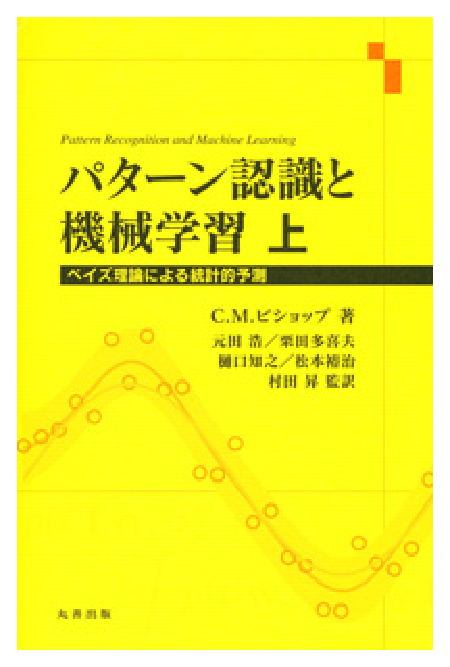
\includegraphics[width=2.5cm,clip]{res/prml.eps}
  \end{figure}
  2$\to$ 2.3.4 
\end{frame}

\section{第$2$章 \enspace 序論}

\end{document}
